\chapter{State of the Art} 

\section{Standard Model}

%\subsection{Higgs Mechanism}

The SM is a theory that explains how the fundamental blocks of the universe interact through the fundamental forces of nature. This model is based on a quantum field theory which incorporates relativity and quantum mechanics. The SM also classifies the fundamental particles and the compound ones. 

According to this model there are two types of fundamental particles in nature: bosons and fermions. Fermions are the particles that compound the matter, while bosons transmit the interactions through their exchange. Bosons have integer spin while fermions have half-integer spin. There are two classifications of fermions: quarks and leptons. The quarks particles have a characteristic property called color charge. There are three types of color charge referred as: blue, red and green. Quarks present a phenomenon called color confinement which causes that they can not be isolated singularly, so they can only be found in nature in group as hadrons. Thus, hadrons are defined as composite subatomic particles and there are two types of them: baryons and mesons. Baryons are conformed by three quarks and mesons by two quarks. The other type of fermions are leptons, which do not posses the color charge property.

The SM explains three fundamental interactions: electromagnetic, strong and weak, but it does not include the gravitational interaction. The electromagnetic interaction acts on particles that have electric charge, it is transmitted by photons, and it has an infinite range. The strong interaction affects color charged particles (quarks) and it is mediated by gluons which carry color charge. The range of strong interaction is just around $10^{-15}$m (the order of the diameter of a medium sized nucleus). The magnitude of strong interaction is big enough to maintain the nucleus of an atom together. The weak interaction appears in the radioactive decay, which is the process responsible for the decay of unstable nucleus. The radioactive decay is caused when there is a greater quanty of protons that of neutrons. The weak force is transmitted through three bosons $W^{\pm}$ and $Z^0$. Since the mass of each of these particles is relatively large, the weak interaction has a short range of around $10^{-18}$ m. 

 \begin{figure}[h] 
 \centering
 \caption{Particles of the Standard Model}
 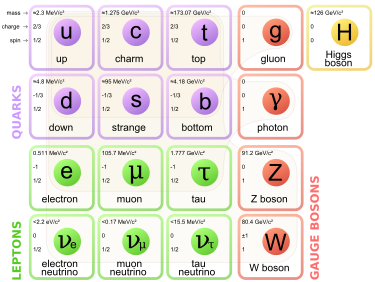
\includegraphics[width=0.4\textwidth]{./Capitulos/StateArt/standard_model} 
 \label{Estandar model}
 \end{figure} 

The Figure \ref{Estandar model} brings together the particles of the SM and specifies their properties. Fermions are grouped into three generations, each having two quarks and two leptons. Each member of a higher generation has a greater mass than the corresponding particle of the previous generation. The classification for quarks is the following: the first generation includes up and down quarks, the second generation strange and charm quarks, and the third generation bottom and top quarks. Each generation contains one quark with charge -1/3 (down-type) and other with charge +2/3 (up-type). For leptons, each generation includes one with -1 charge lepton and one neutral lepton (called neutrino) related to the correspond partner. Their classification is: first generation contains electron and electron neutrino, second muon and muon neutrino, and third tau and tau neutrino. The SM also postulates that for each known particle there exists another particle with the same value of mass and spin but opposite electric charge and different color charge. This partner is called antiparticle.

Additionally, according to the SM, the fundamental particles acquire their mass through their interaction with a scalar field denominated Higgs field. The mediating particle of this field is the Higgs boson and it was discovered on 2012 as announced by the experiments CMS and ATLAS. As it was mentioned earlier, SM is not a complete theory since there are physical phenomena that this theory does not explain. For example, it predicts neutrinos have zero mass but the observations neutrino oscillations indicate the opposite. Moreover, the SM does not provide a possible candidate for DM and does not explain the asymmetry of the neutrinos helicity. For this reason, some theories that extend the reach of SM have been proposed. One simple extension of SM that can explain the smallness of neutrino masses is Type I Seesaw mechanism. 

\section{Neutrinos in the Standard Model}

As it was mentioned earlier, the SM does not explain the reason why the mass of neutrinos is a factor of almost $10^{-6}$ smaller that the mass of the other fermions. Moreover the SM predicts that
the mass of the neutrinos is zero. Addiotionally, it does not provide an explanation to the fact that only left-handed neutrinos have been observed in nature. 
In this section we are going to work on possible solutions to these problems. \footnote{The detailed calculations of the theory explained here are stated in \ref{apendice_neutrinos}}

\subsection{Dirac Mass}

First, we start by studying the Dirac mass term of a free fermion. The Lagrangian equation for a fermion particle is given by the expression:

\begin{equation}
 L = \overline{\psi} \left( i \gamma ^\mu \partial_{\mu} - m \right) \psi \text{,}
\end{equation}

where $\psi$ is the Dirac Spinor. From this Lagrangian expression it is possible to see that in the SM the mass is included through the second term in the equation which is called ``Dirac mass term'':

\begin{equation}
 m \overline{\psi} \psi
\end{equation}

We can write the Dirac Spinor as a sum of its left- and right- chiral states:

\begin{equation}\label{Dirac mass term}
 m \overline{\psi} \psi = m \left( \overbar{\psi_L + \psi_R} \right) \left( \psi_L + \psi_R \right) = m \overline{\psi_L} \psi_R + m \overline{\psi_R}\psi_L
\end{equation} 

In the last expression we used the fact that: $\overline{\psi_L}\psi_L = \overline{\psi_R}\psi_R = 0$ which is proved in Appedix \ref{apendice_neutrinos}. It can be seen from Equation \ref{Dirac mass term} that a massive particle must have both quiral states: left and right. Thus, the Dirac mass can be interpreted as the coupling constant between the two chiral states. Since right-handed 
neutrinos had been never observed in nature, it is expected that neutrinos have zero mass. Although, experiments of neutrino oscillations indicate that neutrinos have a small mass of 
the order of MeV. The former implies either the existence of a right-handed neutrino which is responsible for the mass of the neutrino, or that there exists other sort of mass term.

\subsection{Majorana Mass}

The Majorana Mechanism is based on expressing the mass term in the Lagrangian in only the left-handed chiral state terms.
To do this we start by decomposing the wavefunction into its left and right chiral states in the Dirac Lagrangian: 


\begin{align}
  \phantom{i = j = k}
  &\begin{aligned}
    \mathllap{L} &= \overline{\psi} \left( i \gamma ^\mu \partial_{\mu} - m \right) \psi \\
    \mathllap{}  &= (\overline{\psi_L} + \overline{\psi_R})( i \gamma ^\mu \partial_{\mu} - m)(\psi_L + \psi_R) \\
     \mathllap{} &= i \overline{\psi_L}\gamma^\mu\partial_\mu \psi_L - \overline{\psi_L} m \psi_R +
     i\overline{\psi_R}\gamma^\mu \partial_\mu \psi_R - \overline{\psi_R}m\psi_L
   &\end{aligned}
\end{align}

Since $\overline{\psi_L}\psi_L = \overline{\psi_R}\psi_R = 0$ and $\overline{\psi_R}\gamma^\mu \partial_\mu \psi_L = \overline{\psi_L}\gamma^\mu\partial_\mu \psi_R = 0$
as it is explained in the Appendix \ref{apendice_neutrinos}. Now, we can replace the expression of this Lagrangian in the Euler-Lagrange equation:

\begin{equation}
\frac{\partial L}{\partial (\partial \phi)} - \frac{\partial L}{\partial \phi} = 0
\end{equation}

By doing this we find that the two equations of motion for the fields are two coupled Dirac equations for the right- and left- handed fields:

\begin{equation}\label{majorana_objetive}
i \gamma ^\mu \partial_\mu \psi_L = m \psi_R
\end{equation} 
\begin{equation}\label{majorana_start}
i \gamma ^\mu \partial_\mu \psi_R = m \psi_L
\end{equation} 

In the formulation of the SM the mass of the neutrino is zero, in this case we obtain two equations which are called ``Weyl equations'':
\begin{equation}
i \gamma ^\mu \partial_\mu \psi_L = 0
\end{equation}
\begin{equation}
i \gamma ^\mu \partial_\mu \psi_R = 0
\end{equation}

The former means that neutrinos can be described using two two-component spinors that are helicity eigenstates. These eigenstates represent two states 
with definite and opposite helicity which correspond to the left- and right-handed neutrinos. However, since we have not observed a right-handed neutrino 
we just represent the neutrino as a single left-handed massless field.  \\
\\
Majorana worked out a way to describe a massive neutrino just in terms of it's left-handed field.
This calculation is performed in the Appendix \ref{apendice_neutrinos}. The objective of Majorana was to write the Equation
\ref{majorana_start} as \ref{majorana_objetive} by finding an expression for $\psi_R$ in terms of $\psi_L$. By doing some manipulations of the Equation \ref{majorana_start} we 
find that it can be written as:  

\begin{equation} \label{Equation_not_used}
i \gamma^\mu \partial_\mu C \overline{\psi}^\intercal_R = m C \overline{\psi}^{\intercal}_L \text{,}
\end{equation}

where $C$ is the operator charge conjugation operator. This operator and its properties are explained in Appendix \ref{appendix_charge_conjugation}. Now, the Equation \ref{Equation_not_used} would have the same structure
as Equation \ref{majorana_objetive} if the right-handed term is imposed to be:

\begin{equation} 
\label{Expression_right_handed}
\psi_R = C \overline{\psi}^\intercal_L
\end{equation}

The former assumption requires $C \overline{\psi}^\intercal_L$ to be right-handed, this is proved in the Appendix \ref{apendice_neutrinos}. Thus, the complete Majorana 
field can be written as:
\begin{equation}
\psi = \psi_L + \psi_R = \psi_L + C \overline{\psi}^\intercal_L
\end{equation}

Defining the charge-conjugate field as: $\psi^C_L = C \overline{\psi}^\intercal_L$, we get for the expression of the complete Majorana field:

\begin{equation} \label{Structure_imposed}
\psi = \psi_L + \psi^C_L
\end{equation}

The implications of requiring the right-handed component of $\psi$ to satisfy the Equation                                                    \ref{Structure_imposed} can be studied by taking the charge conjugate of the complete Majorana field. 

\begin{equation}
\psi^C = (\psi_L + \psi^C_L)^C = \psi^C_L + \psi_L = \psi
\end{equation}

Having in mind that the charge conjugation operator turns a particle state into an antiparticle state, it can be deduced that a Majorana particle is its own antiparticle.
Since the charge conjugation operator flips the sign of electric charge, a Majorana particle must be neutral. Thus, the neutrino is the only fermion that could be a Majorana particle.

\subsubsection{Majorana Mass Term}

In Equation \ref{Dirac mass term} we saw that the mass term in the Lagrangian couples the left and right chiral states of the neutrino. Replacing the 
expression we found in Equation \ref{Expression_right_handed} for the right-handed component of the neutrino field in the mass term of the Lagrangian we get the equation \ref{majorana_mass_term}. In this equation we denoted the Dirac Spinor of neutrino as $\nu$. Having in mind that the hermitian conjugated of the first term in the equation is identical, we normalize the Lagrangian and obtain:

%EXPLICAAAAAR expresion y 1/2

\begin{equation}\label{majorana_mass_term}
L_{Maj}^{L} = m \overline{\nu_L} \nu_L^C + m \overline{\nu_L^C} \nu_L = \frac{1}{2} m \overline{\nu_L^{C}} \nu_L
\end{equation}

%EXPLICAR LEPTON NUMBER VIOLATION



\section{Seesaw Mechanism}

As it was mentioned before, in the case that the right-handed chiral field does not exist there can be no Dirac mass term. However, we can have a Majarona mass term in the 
Lagrangian (associated to a left-handed quiral field) so the neutrino would be a Majorana particle:

\begin{equation}
L_{Maj}^{L} = \frac{1}{2} m_L \overline{\nu^{C}}_L \nu_L
\end{equation}

The term $m_L$ is forbidden by electroweak symmetry and it appears after its spontaneous breakdown through the Higgs Mechanism, hence such a term can not exist. In order to let the neutrino to have mass, a right-handed neutrino that interacts only with gravity and the Higgs field must exist.
%EXPLICARRRRRRRRRRRRRRRRRRRRRRRRRRRRRRRRRRRRRRRRRRRRRRRRRR
If we consider that a right-handed chiral neutrino can exist, we would have to add different terms to the Lagrangian. First, if 
we assume that it is possible to write a left-handed Majorana field, we have for the first term:

\begin{equation}
L_L^{M} = m_L \overline{\nu_L} \nu_{L}^C + m_L \overline{\nu_L^C} \nu_L
\end{equation}

Additionally, we have to include a similar term which is the right-handed Majorana field:

\begin{equation}
L_R^{M} = m_R \overline{\nu_R^C} \nu_{R} + m_R \overline{\nu_R} \nu_R^C
\end{equation}

We also have to add Dirac mass terms in order to study the most general Lagrangian: the first Dirac mass term we mentioned on this section (Equation \ref{Dirac normal}) and another one that comes from the 
charge-conjugate fields (Equation \ref{Dirac conjugated}):

\begin{equation}\label{Dirac normal}
L = m_D \overline{\nu_L}\nu_R + m_D \overline{\nu_R}\nu_L
\end{equation} 

\begin{equation}\label{Dirac conjugated}
L = m_D \overline{\nu_R^C} \nu_L^C + m_D \overline{\nu_L^C}\nu_R^C
\end{equation} 

Since the hermitian conjugate of each equation is identical, we can write the most general mass term as a sum ot the Lagrangians we just mentioned:
\begin{equation}
L = \frac{1}{2} \left( m_L \overline{\nu_L^C} \nu_L + m_R \overline{\nu_R^C} \nu_{R} + m_D \overline{\nu_R}\nu_L + m_D \overline{\nu_L^C}\nu_R^C   \right)
\end{equation}

The former equation can be written as a matrix equation: 

\begin{equation}\label{matrix_m_sa}
L_{mass} \propto
\begin{pmatrix} 
  \overline{\nu_L^C} & \overline{\nu_R}
\end{pmatrix}
\begin{pmatrix}
  m_L & m_D \\
  m_D & m_R  
\end{pmatrix}
\begin{pmatrix}
  \nu_L \\
  \nu_R^C  
\end{pmatrix}
\end{equation}

Equation \ref{matrix_m_sa} expresses the Lagrangian in terms of the left and right chiral states. These states do not have a definite mass because the matrix is not diagonal. 
Thus, the left and right chiral states do not correspond to the physical particles (which have a definite mass). Instead the real particles are a superposition of the 
mass eigenstates. In order to find the mass eigenvalues we need to diagonalize the M matrix (the one in the middle of the former equation). This calculation is 
explained in Appendix \ref{apendice_neutrinos}. We find the mass eigenstates are given by the expression:

\begin{equation}
m_{1,2} = \frac{1}{2} \left[ (m_L + m_R) \pm \sqrt{(m_L - m_R)^2 + 4m_D^2} \right]
\end{equation}
 
The fact that the SM does not allow a Majorana left-chiral mass term implies $m_L = 0$. Next, we are going to study the expression of the mass eigenstates $m_1$ and $m_2$. 
When we choose $m_R >> m_D$, we get for the mass eigenvalues:

\begin{equation}
m_1 = \frac{m_D^2}{m_R}
\end{equation}

\begin{equation}
m_2 = m_R \left( 1 + \frac{m_D^2}{m_R^2}\right) \approx m_R 
\end{equation}
 
From both equations above we can deduce that if there a neutrino with mass $m_2$ very large exists, then the other neutrino must have a small mass. 
The former fact is the reason why this mechanism is called ``Seesaw'': the mass of each physical neutrino is controlled by the mass eigenvalues in a way such that when one neutrino is light
the other is heavier. Now, the neutrino mass eigenstates are given by the following expresions:

\begin{equation}
\label{nu_1}
\nu_1 \propto \left( \nu_L + \nu_L^C \right) - \frac{m_D}{m_R^2} \left( \nu_R + \nu_R^C \right)
\end{equation}

\begin{equation}
\label{nu_2}
\nu_2 \propto \left( \nu_R + \nu_R^C \right) + \frac{m_D}{m_R^2} \left( \nu_L + \nu_L^C \right)
\end{equation}

The Equations \ref{nu_1} and \ref{nu_2} show that $\nu_1$ is mostly the left-handed light Majorana neutrino while $\nu_2$ is the heavy sterile right-handed neutrino. This is the explanation 
that the Seesaw Mechanism gives to the fact that the neutrino is much lighter than the other fermions. 
 
 
 
 
 
 